\documentclass[12pt, a4paper]{article}

% Ru lang stuff
\usepackage [utf8x] {inputenc}
\usepackage [T2A] {fontenc}

% running titles 
\usepackage{fancybox}
\usepackage{fancyhdr}

% for last page number
\usepackage{lastpage}

%for colored tablets cells
\usepackage{colortbl}

% for Ru text in formulas
\usepackage[warn]{mathtext}

% for captions 
\usepackage[labelsep=period]{caption}

% for colored hyperrefs
\usepackage{xcolor}
\usepackage{hyperref}

% for pictures 
\usepackage{graphicx}

% for coll math
\usepackage{amsmath}

% path to all pictures
\graphicspath{{picks/}}

% for enumerates
\usepackage[shortlabels]{enumitem}

% for diff running titles on pages with diff parity
\usepackage{ifthen}
\usepackage{pdfpages}
\usepackage[strict]{changepage}

%for drawings
\usepackage{tikz}
\usetikzlibrary{calc}
\usetikzlibrary{decorations.pathmorphing}

% for good text in tablets
\usepackage{array}

% upgrading tables
\newcolumntype{P}[1]{>{\centering\arraybackslash}p{#1}}
\newcolumntype{M}[1]{>{\centering\arraybackslash}m{#1}}


% dock fields 20 15 15 35
\usepackage[left=12mm, top=12mm, right=15mm, bottom=28mm, nohead, footskip=10mm]{geometry}

% for cool tables
\usepackage{multirow}

% for different section/subsection/subsubsection styles in contents and doc
\usepackage[english, russian]{babel}

\usepackage{amsmath}

% for cool tables
\usepackage{tabularx}

\newcommand{\sect}[2] {
    \addtocounter{section}{1}
    \section*{\Huge\thesection.\,#1}
    \addcontentsline{toc}{subsection}{ \texorpdfstring{\thesection.\qquad\qquad #2}{Lg}}
}

\newcommand{\subsec}[2] {
    \addtocounter{subsection}{1}
    \subsection*{\thesubsection.\,#1}
    \addcontentsline{toc}{subsection}{ \texorpdfstring{\quad \thesubsection.\qquad\ #2}{Lg}}
}

\newcommand{\subsubsec}[2] {
    \addtocounter{subsubsection}{1}
    \subsubsection*{\thesubsubsection.\,#1}
    \addcontentsline{toc}{subsection}{ \texorpdfstring{\quad\quad\ \thesubsubsection. #2}{Lg}}
}
%-------------------------------------------------------------------------%

% for easy mini pages with shifts
\newcommand{\shiftedText}[3]{
\hspace*{#1}\begin{minipage}[t]{#2}
#3
\end{minipage}
}

\newcolumntype{P}[1]{>{\centering\arraybackslash}p{#1}}

% page style setup (for running titles)
\fancypagestyle{plain}{ %
\fancyhf{} % remove everything

 % lines parameters
\renewcommand{\headrulewidth}{0pt}
\renewcommand{\footrulewidth}{0pt}

% running titles contents
\fancyfoot[L]{\ifthenelse{\isodd{\thepage}}{Работа 1.1.1}{\thepage}}
\fancyfoot[R]{\ifthenelse{\isodd{\thepage}}{\thepage}{Работа 1.1.1}}
}

% choosing page style with our running titles
\pagestyle{plain}

\tolerance = 10000

\title{Лабораторная работа №1.1.1.}
\author{Mikhail Pavlov \thanks{MIPT}}
\date{September, 2021}
\begin{document}

\shiftedText{0.5cm}{14cm}
{
    \begin{center}
    \vspace*{1.0cm}    
        
        {\bf\huge Работа 1.1.1 }
        
    \vspace*{0.2cm}    
        
        {\bf\Large Определение систематических и случайных погрешностей при измерении удельного сопротивления проволоки }
        
    \vspace*{0.8cm}
        {\Large Работу выполнил Павлов Михаил Б01-109 }
        
    \vspace*{1.6cm}
    
    \end{center}
    
    {\bf\noindent Цель работы: }  Измерить удельное сопротивление проволоки и вычислить систематические и случайные погрешности при использовании таких измерительных приборов, как линейка, штангенциркуль, микрометр, амперметр, вольтметр и мост постоянного тока.
    
    \vspace*{0.6cm}
    
    {\bf\noindent В работе используются: } линейка, штангенциркуль, микрометр, отрезок проволоки из нихрома, амперметр, вольтметр, источник ЭДС, мост постоянного тока, реостат, ключ.

}

\fancypagestyle{plain}{ %
\fancyhf{} % remove everything

 % lines parameters
\renewcommand{\headrulewidth}{0pt}
\renewcommand{\footrulewidth}{0pt}

% running titles contents
\fancyfoot[L]{\ifthenelse{\isodd{\thepage}}{Работа 1.1.1}{\thepage}}
\fancyfoot[R]{\ifthenelse{\isodd{\thepage}}{\thepage}{Работа 1.1.1}}
}

% choosing page style with our running titles
\pagestyle{plain}

\tolerance = 10000

\newpage

        {\large 1. Аннотация \\}

            В работе измеряется удельное сопротивление тонкой проволоки круглого сечения, изготовленной из нихромового сплава. Используются следующие методы измерений сопротивления:
        1) определение углового коэффициента наклона зависимости напряжения на проволоке от тока
        через неё, измеряемых с помощью аналоговых и цифровых вольтметров и амперметров, 2) измерение с помощью моста постоянного тока. Геометрические размеры образца измеряются с
        помощью линейки, штангенциркуля и микрометра. Детально исследуется систематические и
        случайные погрешности проводимых измерений. \\

        {\large 2. Теоретические сведения \\}

        Удельное сопротивление однородной проволоки круглого сечения, имеющей всюду одинаковую толщину: \\
        \begin{equation}
            \rho = R \frac{\pi d^2}{4l},
        \end{equation}
где $𝑅$ — сопротивление проволоки, $d$ — её диаметр, $𝑙$ — длина.
    Согласно закону Ома напряжение $𝑉$ и ток $𝐼$ в образце связаны соотношением
\begin{equation}
    V = RI.
\end{equation}

\noindent\begin{minipage}[c]{0.67\textwidth}
    \hspace{1cm}Для измерения напряжения и тока использовалась схема рис. 1.
    Ввиду неидеальности используемого вольтметра необходимо
учесть поправку на его конечное сопротивление $𝑅_𝑉$. Показания амперметра $I_A$ и вольтметра $V_B$ связаны соотношением
\begin{equation}
    V_B = R'I_A,
\end{equation}
где $𝑅′$ — сопротивление параллельно соединенных проволоки и
вольтметра, причём $\frac{1}{R'} = \frac{1}{R} + \frac{1}{R_V},$ и $R_V >> R, R'$. График зависимости
$𝑉_B (𝐼_A)$ должен представлять прямую, угловой коэффициент которой есть $𝑅′$, откуда сопротивление образца может быть найдено как
\begin{displaymath}
    R =\frac{R_V R'}{R_V - R'} \approx R'(1 + \frac{R'}{R_V}).
\end{displaymath}
\end{minipage}
\begin{minipage}[c]{0.32\textwidth}
    \begin{center}
        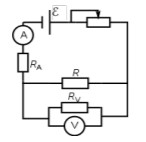
\includegraphics[scale=1]{Pics/scheme1.jpg} \\
        \textit{\textcolor[HTML]{000000}{Рис. 1. Схема измерения \\ вольт-амперной характе- \\ ристики проволоки}}
    \end{center}
\end{minipage}

\vspace*{0.5cm}
{\large 3. Инструментальные погрешности \\} \\
\textbf{Линейка: } $\Delta_{rul} \approx \pm 2$ мм. с учётом погрешности $\pm 0.5$ мм. (половина цены деления линейки) и неидеальное расположение линейки относительно проволоки. \\
\textbf{Штангенциркуль: } $\Delta_{cal} = \pm 0.05$ мм (маркировка производителя)                                                                                                  \\
\textbf{Микрометр: } $\Delta_{mcm} = \pm 0.01$ мм (маркировка производителя)                                                                                                      \\    
\textbf{Вольтметр: } Характеристика вольтметра:
                                                                                                                                                            \\      
\begin{center}
\begin{tabular}{ | p{6cm} | p{3.2cm} | p{3cm} | }
    \hline
 Предел измерений & 10 B \\ \hline
 Внутреннее сопротивление & $R_V = 10$ МОм \\ \hline
\end{tabular}
\end{center} 

\newpage
\noindent\textbf{Амперметр: } Характеристика амперметра:                                                                                                                                                   \\      
\begin{center}
\begin{tabular}{ | p{6cm} | p{3.2cm} | p{3cm} | }
    \hline
    Класс точности & 0.2 \\  \hline
 Предел измерений & 0.75 А \\ \hline
 Внутреннее сопротивление & $R_A = 116$ мОм \\ \hline
 Погрешность & $\pm$ 1.5 мА (0.2\%) \\ \hline   
\end{tabular}
\end{center} 
\vspace*{0.3cm}

{\large 4. Результаты измерений и обработка данных \\} 

Измерение диаметра проволоки c помощью \textbf{микрометра}:
\begin{center}
    \begin{tabular}{ |c|c|c|c|c|c|c| } \hline
        N & 1 & 2 & 3 & 4 & 5 & 6 \\
        \hline
        $d_1$, мм & 0.38 & 0.37 & 0.38 & 0.37 & 0.38 & 0.38 \\
        \hline
    \end{tabular}
    \end{center} 

    Измерение диаметра проволоки c помощью \textbf{штангенциркуля}:
\begin{center}
    \begin{tabular}{ |c|c|c|c|c|c|c| } \hline
        N & 1 & 2 & 3 & 4 & 5 & 6 \\
        \hline
        $d_2$, мм & 0.4 & 0.4 & 0.4 & 0.4 & 0.4 & 0.4 \\
        \hline
    \end{tabular}
    \end{center} 

    Получаем $<\overline{d_1}> = 0.377$ мм и $<\overline{d_2}> = 0.4$ мм

    При измерении диаметра проволоки штангенциркулем случайная погрешность измерения отсутствует. Следовательно, точность измерения определяется только точностью штангенциркуля (систематической погрешностью): $d_2 = (0.40 \pm 0.05)$ мм \\
    Измерения с помощью микрометра содержат как систематическую, так и случайную погрешности. \\
    $\sigma_{sys}$ = 0.01мм, $\sigma_{ran} = \frac{1}{N} \sqrt{\sum_{i = 1}^{n} (d - <\overline{d}>)^2 \approx 1.5 * 10^{-3}}$ мм \\
    Поскольку $\sigma_{sys}^2 >> \sigma_{ran}^2$, то можно считать проволоку однородной по диаметру, а погрешность определить только лишь систематической погрешностью микрометра. \\
    
    \textbf{Вычисление площади поперечного сечения:} \\
    $S = \frac{\pi d^2}{4} = \frac{3.14 * (3.77 * 10^{-1})^2}{4} = 1.12 * 10^{-3}$ см$^2$ \\
    Теперь вычислим погрешность: \\
    $\sigma_S = 2 \frac{\sigma_d}{<d>}S = 2 \frac{0.01}{0.377} * 1.12 * 10^{-3} \approx 5.9 * 10^{-5}$ см$^2$ \\
    Таким образом, $S = (1.12 \pm 0.06) * 10^{-3}$ см$^2$ \\
    
    \textbf{Измерение силы тока и напряжения:} \\
    Соберём схему, указанную на рисунке, и проведём опыт для трёх длин проволоки $l_1 = 20$см, $l_2 = 30$см и $l_3 = 50$см. Системная погрешность измерения длины проволоки равна 0.2см. \\
    \\ l = 20см:
    \begin{center}
        \begin{tabular}{ |c|c|c|c|c|c|c|c|c|c|c|c|c| } \hline
            N & 1 & 2 & 3 & 4 & 5 & 6 & 7 & 8 & 9 & 10 & 11 & 12 \\ \hline
            $I$, A & 0.135 & 0.155 & 0.180 & 0.240 & 0.360 & 0.675 & 0.655 & 0.430 & 0.295 & 0.220 & 0.150 & 0.110 \\ \hline
            $U$, B & 0.268 & 0.305 & 0.355 & 0.481 & 0.730 & 1.365 & 1.321 & 0.867 & 0.595 & 0.445 & 0.375 & 0.271 \\ \hline
            $I$, дел & 27 & 31 & 36 & 48 & 72 & 135 & 131 & 86 & 59 & 44 & 30 & 22 \\ \hline
        \end{tabular}
        \end{center}
    l = 30см:
    \begin{center}
        \begin{tabular}{ |c|c|c|c|c|c|c|c|c|c|c|c|c| } \hline
            N & 1 & 2 & 3 & 4 & 5 & 6 & 7 & 8 & 9 & 10 & 11 & 12 \\ \hline
            $I$, A & 0.150 & 0.165 & 0.200 & 0.265 & 0.360 & 0.735 & 0.695 & 0.480 & 0.320 & 0.190 & 0.160 & 0.120 \\ \hline
            $U$, B & 0.466 & 0.524 & 0.617 & 0.834 & 1.131 & 2.363 & 2.224 & 1.517 & 1.010 & 0.592 & 0.506 & 0.379 \\ \hline
            $I$, дел & 30 & 33 & 40 & 53 & 72 & 147 & 139 & 96 & 64 & 38 & 32 & 24 \\ \hline
        \end{tabular}
        \end{center}
    l = 50см:
    \begin{center}
        \begin{tabular}{ |c|c|c|c|c|c|c|c|c|c|c|c|c| } \hline
            N & 1 & 2 & 3 & 4 & 5 & 6 & 7 & 8 & 9 & 10 & 11 & 12 \\ \hline
            $I$, A & 0.100 & 0.115 & 0.130 & 0.150 & 0.165 & 0.370 & 0.420 & 0.375 & 0.320 & 0.220 & 0.150 & 0.110 \\ \hline
            $U$, B & 0.516 & 0.607 & 0.689 & 0.774 & 0.867 & 1.942 & 2.205 & 1.954 & 1.685 & 1.144 & 0.79 & 0.567 \\ \hline
            $I$, дел & 20 & 23 & 26 & 30 & 33 & 74 & 84 & 75 & 64 & 44 & 30 & 22 \\ \hline
        \end{tabular}
        \end{center}

    \textbf{Измерение сопротивления проволоки:} \\
    Результаты измерений зависимостей показаний вольтметра $V_B$ от показаний амперметра $𝐼_A$ в
    схеме рис. 1 при разных длинах 𝑙 образца представлены в таблицах выше. Соответствующие графики
    зависимостей изображены на рис. 2. \\

    \begin{minipage}[c]{1\textwidth}
        \begin{center}
            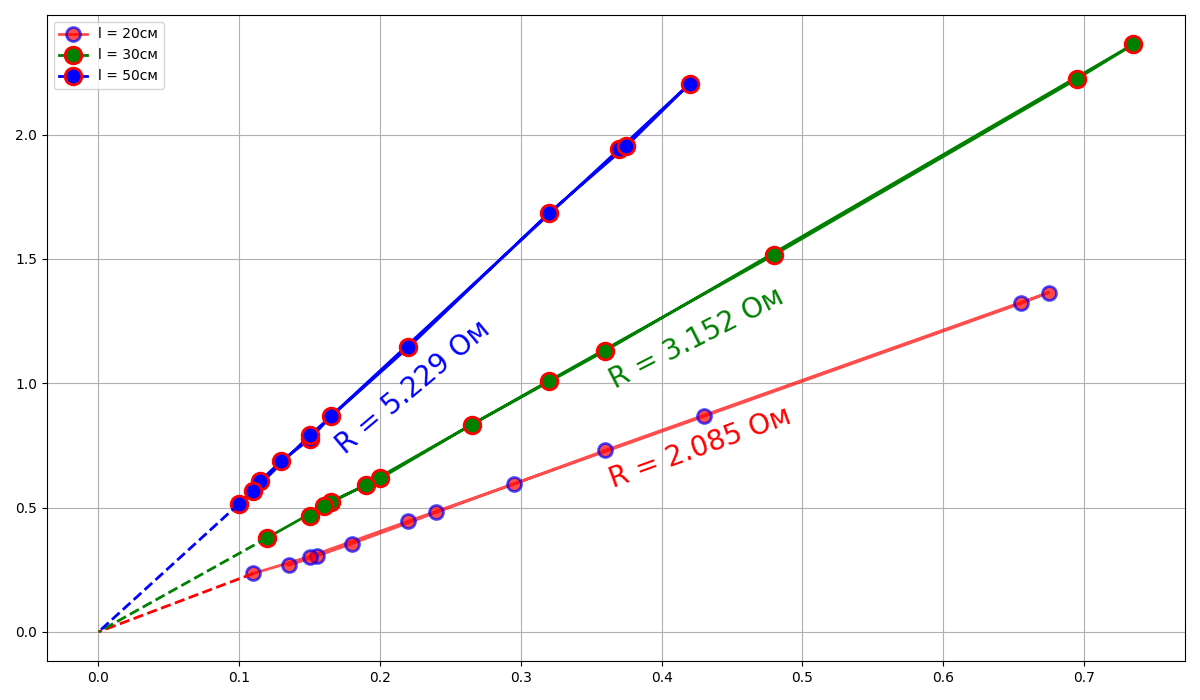
\includegraphics[scale=0.4]{Pics/1.1.1.png} \\
            \textit{\textcolor[HTML]{000000}{Рис. 2. Графики зависимости I от U при различных значениях R }}
        \end{center}
    \end{minipage}
    \vspace*{0.6cm}

    По графику убеждаемся, что экспериментальные данные с хорошей точностью (в пределах
    инструментальных погрешностей опыта) ложатся на теоретическую прямую 𝑉 = 𝑅I, исходящую из начала координат. \\
    Пользуясь методом наименьших квадратов, строим аппроксимирующие прямые $V_B = \overline{R}I_A$, определяя их угловой коэффициент по формуле 
    \begin{equation}
        \overline{R} = \frac{<VI>}{<I^2>}.
    \end{equation}                                                                                                                                                    
    Случайную погрешность определения углового коэффициента вычисляем как
    \begin{displaymath}
        \sigma_{R}^{ran} = \sqrt{\frac{1}{n-1} (\frac{<V^2>}{<I^2>} - \overline{R}^2)}
    \end{displaymath}
    Оценим возможную систематическую погрешность, обусловленную инструментальными
погрешностями приборов. Предполагая, что при всех измерениях относительная погрешность
приборов одинакова, оценим погрешность вычисления частного 𝑅 = 𝑉/𝐼 при максимальных
значениях 𝑉 и 𝐼:
    \begin{displaymath}
        \Delta_{R}^{sys} ~ R \sqrt{(\frac{\Delta_V}{V_{max}})^2 + (\frac{\Delta_I}{I_{max}})^2}.
    \end{displaymath}
    Полная погрешность измерения R не превосходит значения
    \begin{displaymath}
        \sigma_{R}^{full} \leq \sqrt{(\sigma_{R}^{ran})^2 + (\Delta_{R}^{sys})^2}.
    \end{displaymath}
    Результаты сведены далее в таблице. Там же для сравнения приведены результаты измерения R с помощью моста Уинстона.
    \begin{center}
        \begin{tabular}{ |c|c|c|c|c|c| } \hline
            l, см & $\overline{R}$, Ом & $\sigma_{R}^{ran}$, Ом & $\Delta_{R}^{sys}$, Ом & $\sigma_{R}^{full}$, Ом & $R_b$, Ом \\ \hline
            50 & 5.229 & 0.016 & 0.034 & 0.037 & $5.351 \pm 0,010$ \\ \hline
            30 & 3.152 & 0.017 & 0.022 & 0.026 & $3.227 \pm 0,010$ \\ \hline
            20 & 2.085 & 0.019 & 0.014 & 0.017 & $2.153 \pm 0,010$ \\ \hline
        \end{tabular}
        \end{center} 
Случайная составляющая измерения сопротивления мала, а основной вклад вносят систематические приборные погрешности. Контрольные измерения с помощью моста дают
завышенные результаты, но все отклонения находятся в пределах $\pm 2\sigma_{R}^{full}$.
полн. \\

\textbf{Вычисление удельного сопротивления:} \\
По формуле (1) находим удельное сопротивление материала проволоки, используя значения
$\overline{R}$, полученные выше. Сравнивая относительные величины погрешностей величин, входящих в
(1), приходим к выводу, что наибольший вклад в погрешность вносит измерение диаметра проволоки $(2\sigma_d/d ∼ 5.6\%)$, при этом вкладом остальных измерений можно пренебречь: $\sigma_{\rho} \approx \frac{2\sigma_d}{d} \rho$.
\begin{center}
    \begin{tabular}{ |c|c| } \hline
        N опыта & $\rho, 10^{-6}$ Ом * м \\ \hline
        1 & $(1.167 \pm 0.065) * 10^{-6}$ Ом * м \\ \hline
        2 & $(1.172 \pm 0.065) * 10^{-6}$ Ом * м \\ \hline
        3 & $(1.164 \pm 0.065) * 10^{-6}$ Ом * м \\ \hline
    \end{tabular}    
\end{center}

Усредняя результаты опытов, окончательно получим: \\
    $\underline{\overline{\rho} = (1.17 \pm 0.07) * 10^{-6}}$ Ом * м \\
    
    {\large 5. Обсуждение результатов и выводы \\}
    Вклад погрешности измерения площади проволоки $~6\%$, что является основной частью погрешности. Значит, для измерения сопротивления достаточна точность $3-4\%$ \\
    Полученное значение сравнимо с табличным значением удельного сопротивления нихрома. Табличное значение = $1.1 * 10^{-6}$ Ом * м, что лежит в пределах нашей погрешности, откуда следует, что результаты равны. \\
    Мы измерили удельное сопротивление проволоки и вычислили систематические и случайные погрешности.


\end{document}